\documentclass[a4paper,10pt,reqno]{article}

\usepackage{gensymb}
\usepackage[margin=0.95in]{geometry}
\usepackage{mathtools,graphicx}
\usepackage{float}
\usepackage{siunitx}
\usepackage{subfig}
\usepackage{amsmath,amsfonts,amssymb,amsthm,mathrsfs,bm}
\usepackage[outdir=../]{epstopdf}
\usepackage{inputenc}
\usepackage{sidecap}
\usepackage{caption}
\usepackage{hyperref}

\usepackage{array}
\usepackage{booktabs}
\usepackage{listings}
\usepackage{color}
\usepackage[dvipsnames]{xcolor}
\usepackage{tcolorbox}
\usepackage{textcomp}


% --------------------------------------------------------
% Custom Colours
% --------------------------------------------------------
\definecolor{CommentGreen}{rgb}{0.0,0.4,0.0}
\definecolor{Background}{rgb}{0.9,1.0,0.85}
\definecolor{lrow}{rgb}{0.914,0.918,0.922}
\definecolor{drow}{rgb}{0.725,0.745,0.769}


% --------------------------------------------------------
% Typesetting Python code
% --------------------------------------------------------
\lstloadlanguages{Python}%
\lstset{
    language=Python, upquote=true, frame=single,
    basicstyle=\small\ttfamily,
    backgroundcolor=\color{yellow!30},
    keywordstyle=[1]\color{NavyBlue}\bfseries,
    keywordstyle=[2]\color{RubineRed},
    keywordstyle=[3]\color{orange!90}\bfseries,
    keywordstyle=[4]\color{Green!90}\bfseries,
    identifierstyle=,
    commentstyle=\usefont{T1}{pcr}{m}{sl}\color{MidnightBlue}\small,
    stringstyle=\color{purple},
    showstringspaces=false, tabsize=4, morekeywords={import,as},
    morekeywords=[2]{args,__init__},
    morekeywords=[3]{@property},
    morekeywords=[4]{self},
    morecomment=[l][\color{blue}]{...},
    escapeinside={(@*}{*@)},
    numbers=none, firstnumber=1,
    numberstyle=\tiny\color{blue},
    stepnumber=1, xleftmargin=10pt, xrightmargin=10pt
}

\synctex=1

\hypersetup{
    unicode=false, pdftoolbar=true, 
    pdfmenubar=true, pdffitwindow=false, pdfstartview={FitH}, 
    pdftitle={ELE2024 Coursework}, pdfauthor={A. Author},
    pdfsubject={ELE2024 coursework}, pdfcreator={A. Author},
    pdfproducer={ELE2024}, pdfnewwindow=true,
    colorlinks=true, linkcolor=red,
    citecolor=blue, filecolor=magenta, urlcolor=cyan
}

% --------------------------------------------------------
% CUSTOM COMMANDS
% --------------------------------------------------------
\renewcommand{\Re}{\mathbf{re}}
\renewcommand{\Im}{\mathbf{im}}
\newcommand{\R}{\mathbb{R}}
\newcommand{\N}{\mathbb{N}}
\newcommand{\C}{\mathbb{C}}
\newcommand{\lap}{\mathscr{L}}
\newcommand{\dd}{\mathrm{d}}
\newcommand{\smallmat}[1]{\left[ \begin{smallmatrix}#1 \end{smallmatrix} \right]}

\numberwithin{equation}{section}
\graphicspath{ {../Figures/} }
\hyphenpenalty=10000

% --------------------------------------------------------
% Opening: Title and Author Names
% --------------------------------------------------------
\title{Inverted Pendulum Lab}
\author{Allwyn Bino}
\date{}

\begin{document}
\maketitle

\section{Question 1}

\noindent
$\phi$ and $\psi$ represent part of the State Space Representation of the Inverted Pendulum.\\
$\phi$ and $\psi$ are derivated to Linearise the system.\\
The following code was written, to calculate the partial deriviatives of $\phi(F, x_{3}, x_{4})$, and $\psi(F, x_3, x_4)$,
with respect to $F, x_3, x_4$.\\

\begin{lstlisting}[language=Python]
# Evaluate expressions at F=0, x3=0 and x4=0
def evaluate_at_equilibrium(equation):
    return equation.subs([(F, 0), (x3, 0), (x4, 0)])

#Defining Symbols
M, m, ell, g, x1, x2, x3, x4, F = sym.symbols('M, m, ell , g, x1 , x2 , 
									x3 , x4 , F')
phi_numer = 4 * m * ell * x4 ** 2 * sym.sin(x3) + 4 * F - 3 * m * g \
           * sym.sin(x3) * sym.cos(x3)
phi_denom = 4 * (M + m) - 3 * m * sym.cos(x3) ** 2
phi = phi_numer / phi_denom  # Equation for Phi

psi_numer = m * ell * x4 ** 2 * sym.sin(x3) * sym.cos(x3) + F * sym.cos(x3) \
            - (M + m)  * g * sym.sin(x3)
psi_denom = (4 * (M + m) - 3 * m * sym.cos(x3) ** 2) * ell
psi = -3 * psi_numer / psi_denom  # Equation for Psi

# Used to get properly formatted LaTeX output
functions = (phi, psi)
str_functions = ("phi", "psi")
equilibriate_at = (F, x3, x4)

answers_diff = []  # Holds all the equilibrated values

# Computing derivatives of phi and psi at the equilibrium point
for function in functions:
    derivative_answer = []
    for value in equilibriate_at:
        # Computing each derivative at the equilibrium point
        diff = evaluate_at_equilibrium(function.diff(value))
        derivative_answer.append(diff)
    answers_diff.append(derivative_answer)

for x in range(len(answers_diff)):
    for y in range(len(answers_diff[x])):
        # Generating LaTeX
        print("\\frac{\\partial \\" + str_functions[x]
              + f"{equilibriate_at}"+"}{\\partial " 
              + sym.latex(equilibriate_at[y])
              + "}" + f" &= {sym.latex(answers_diff[x][y])}\\\")
\end{lstlisting}

\newpage
\noindent
The following was the output.\\
Since the outputs are constant, they can be assigned a variable, to make equations look neater.

\begin{align}
\frac{\partial \phi(F, x_3, x_4)}{\partial F} &= \frac{4}{4 M + m} = a\cr
\frac{\partial \phi(F, x_3, x_4)}{\partial x_{3}} &= - \frac{3 g m}{4 M + m} = b\cr
\frac{\partial \phi(F, x_3, x_4)}{\partial x_{4}} &= 0\cr
\\
\frac{\partial \psi(F, x_3, x_4)}{\partial F} &= - \frac{3}{\ell \left(4 M + m\right)} = c\cr
\frac{\partial \psi(F, x_3, x_4)}{\partial x_{3}} &= \frac{3 g \left(M + m\right)}{\ell \left(4 M + m\right)} = d\cr
\frac{\partial \psi(F, x_3, x_4)}{\partial x_{4}} &= 0\cr
\end{align}


\section{Question 2}
The Linearised System is represented by the following equations.
\begin{align}
\dot{x_1} &= x_{2}\\
\dot{x_2} &= F a - b x_{3}\\
\dot{x_3} &= x_{4}\\
\dot{x_4} &= - F c + d x_{3}
\end{align}

\noindent
These Linearised equations can be Laplaced, so that their Transfer Function can be determined. After that, the system can be simulated with all kinds of input.\\
The Laplaced Equations are as follows.
\begin{align}
X_{1} s &= X_{2}\\
X_{2} s &= a F_{lap} - b X_{3}\\
X_{3} s &= X_{4}\\
X_{4} s &= -c F_{lap} + d X_{3}
\end{align}

\noindent
To get the Transfer Function, $G_{\theta}$, with input $F_{lap}$, and output $X_3$, substitute (2.7) into (2.8), then rearrange.
\begin{align}
X_{4} s &= -c F_{lap} + d X_{3}\cr
\left( X_{3} s \right) s &= -c F_{lap} + d X_{3}\cr
X_{3}  s^2 &= -c F_{lap} + d X_{3}\cr
X_{3}  s^2 - d X_{3} &= -c F_{lap}\cr
X_{3} \left( s^2 - d \right) &= -c F_{lap}\cr
\frac{X_{3}}{F_{lap}} &= \frac{-c}{s^2 - d}\\
G_{\theta} = &= \frac{-c}{s^2 - d}
\end{align}

\newpage
\noindent
To get $G_x$, with input $F_{lap}$, and output $X_1$, sustitute (2.5) into (2.6), then rearrange (2.9), to get an equation for $X_3$. Then substitue this into Equation (2.6).
\begin{align}
X_{2} s &= a F_{lap} - b X_{3}\cr
\left( X_{1} s \right) s &= a F_{lap} - b \left( \frac{-c}{s^2 - d} F_{lap} \right)\cr
X_{1} s^2 &= a F_{lap} + \frac{bc}{s^2 - d} F_{lap} \cr
X_{1} s^2 &= \left( a + \frac{bc}{s^2 - d} \right) F_{lap} \cr
\frac{X_{1}}{F_{lap}} &= \frac{a}{s^2} + \frac{bc}{s^2 \left( s^2 - d \right)}\\
G_{x} &= \frac{a}{s^2} + \frac{bc}{s^2 \left( s^2 - d \right)}
\end{align}

\noindent
The second fraction in $G_x$ can be expanded, by Partial Fraction Decomposition.
\begin{align}
\frac{1}{s^2 \left( s^2 - d \right)} &= \frac{A_1 s + A_2}{s^2} + \frac{B_1 s + B_2}{s^2 - d}
\end{align}

\noindent
Solving for $A_1$, $A_2$, $B_1$, and $B_2$ gives these values.
\begin{align}
1 &= \left( A_1 s + A_2 \right) \left(s^2 - d\right) + \left( B_1 s + B_2 \right) \left(s^2 \right) \cr
1 &= A_1 s^3 + A_2 s^2 - d A_1 s - d A_2 + B_1 s^3 + B_2 s^2\\
\cr
0 s^3 &= \left( A_1 + B_1 \right) s^3 \cr
0 &= A_1 + B_1 \\
\cr
0 s^2 &= \left( A_2 + B_2 \right) s^2 \cr
0 &= A_2 + B_2 \\
\cr
0 s &= \left( -d A_1 \right) s\cr
0 &= -d A_1 \cr
0 &= A_1 \therefore B_1 = 0 \\
\cr
1 &= -d A_2 \cr
\frac{-1}{d} &= A_2 \therefore B_2 = \frac{1}{d}
\end{align}

\noindent
Substituting these value into (2.12) gives the follwoing equation for $G_x$.
\begin{align}
G_{x} &= \frac{a}{s^2} + bc \frac{A_1 s + A_2}{s^2} + bc \frac{B_1 s + B_2}{s^2 - d}\cr
G_{x} &= \frac{a}{s^2} + bc \frac{\frac{-1}{d}}{s^2} + bc \frac{\frac{1}{d}}{s^2 - d}\cr
G_{x} &= \frac{a}{s^2} - \frac{bc}{d s^2} + \frac{bc}{ds^2 - d^2}
\end{align}

\newpage
\section{Question 3}
Now that the Transfer Functions have been determined, the Impulse, Step and Frequencey Response of the system can be simulated.
The following code was written to compute the Impulse, Step and Frequency Response of the Transer Functions, 
$G_{\theta}$ and $G_x$.

\begin{lstlisting}[language=Python]
a, b, c, d = sym.symbols("a, b, c, d", real=True, positive=True)  # Constants

# Transfer Function with F_lap as input
G_theta = -c / (s ** 2 - d)  # Output is X3
G_x = a / (s ** 2) \
      + b * c / (d * (s ** 2 - d)) \
      - b * c / (d * s ** 2)  # Output is X1

transfers = [G_theta, G_x]  # Transfer Functions
str_transfers = ["G_{\\theta}", "G_x"]  # Transfer Function Names

omega = sym.symbols("w", real=True)

# Impulse Response is F_lap = 1 in s-domain
# Step Response is F_lap = 1/s in s-domain
# Frequency Response is F = sin(wt) in t-domain for this particular example
# Frequency Response is F_lap = (w**2 / (s**2 + w**2) in s-domain
inputs = [(1), (1 / s), (omega**2 / (s ** 2 + omega ** 2))]
str_inputs = ["Impulse Response", "Step Response", "Frequency Response"]

for x in range(len(transfers)):
    G = transfers[x]  # Each Transfer Function
    str_G = str_transfers[x]  # Name of Transfer Function

    for y in range(len(inputs)):
        F_lap_in = inputs[y]

        # Laplace Output
        lap_output = G * F_lap
        lap_output = lap_output.subs(F_lap, F_lap_in).simplify()

        # Time Domain Output
        output = (sym.inverse_laplace_transform(lap_output, s, t)).simplify()

        # Creating LaTeX Output
        print(str_inputs[y] + f" of ${str_G}$: ")
        print("\\[" + str_G + "\\times" + sym.latex(F_lap_in) + "=" 
              + sym.latex(lap_output) + "\\]")
        print("\\[ \lap^{-1} \\{" + str_G + "\\times" + sym.latex(F_lap_in)
              + "\\} (t) =" + sym.latex(output) + "\\]")
\end{lstlisting}

\noindent
The following was the output.

\noindent
Impulse Response of $G_{\theta}$: 
\begin{align}G_{\theta}\times1=\frac{c}{d - s^{2}}\end{align}
\begin{align} \lap^{-1} \{G_{\theta}\times1\} (t) =- \frac{c \sinh{\left(\sqrt{d} t \right)}}{\sqrt{d}}\end{align}
Step Response of $G_{\theta}$: 
\begin{align} G_{\theta}\times\frac{1}{s}=\frac{c}{s \left(d - s^{2}\right)}\end{align}
\begin{align} \lap^{-1} \{G_{\theta}\times\frac{1}{s}\} (t) =- \frac{2 c \sinh^{2}{\left(\frac{\sqrt{d} t}{2} \right)}}{d}\end{align}
Frequency Response of $G_{\theta}$: 
\begin{align} G_{\theta}\times\frac{w^{2}}{s^{2} + w^{2}}=\frac{c w^{2}}{\left(d - s^{2}\right) \left(s^{2} + w^{2}\right)}\end{align}
\begin{align} \lap^{-1} \{G_{\theta}\times\frac{w^{2}}{s^{2} + w^{2}}\} (t) =\frac{c w \left(2 d^{\frac{3}{2}} e^{\sqrt{d} t} \sin{\left(t w \right)} + 2 \sqrt{d} w^{2} e^{\sqrt{d} t} \sin{\left(t w \right)} - d w e^{2 \sqrt{d} t} + d w - w^{3} e^{2 \sqrt{d} t} + w^{3}\right) e^{- \sqrt{d} t}}{2 \sqrt{d} \left(d^{2} + 2 d w^{2} + w^{4}\right)}\end{align}
Impulse Response of $G_x$: 
\begin{align} G_x\times1=\frac{- a d + a s^{2} + b c}{s^{2} \left(- d + s^{2}\right)}\end{align}
\begin{align} \lap^{-1} \{G_x\times1\} (t) =\frac{a \sinh{\left(\sqrt{d} t \right)} - \sqrt{d} \left(a d - b c\right) \left(- \frac{t}{d} + \frac{\sinh{\left(\sqrt{d} t \right)}}{d^{\frac{3}{2}}}\right)}{\sqrt{d}}\end{align}
Step Response of $G_x$: 
\begin{align} G_x\times\frac{1}{s}=\frac{- a d + a s^{2} + b c}{s^{3} \left(- d + s^{2}\right)}\end{align}
\begin{align} \lap^{-1} \{G_x\times\frac{1}{s}\} (t) =\frac{2 a \sinh^{2}{\left(\frac{\sqrt{d} t}{2} \right)} + \frac{\left(a d - b c\right) \left(\frac{d t^{2}}{2} - \cosh{\left(\sqrt{d} t \right)} + 1\right)}{d}}{d}\end{align}
Frequency Response of $G_x$: 
\begin{align} G_x\times\frac{w^{2}}{s^{2} + w^{2}}=\frac{w^{2} \left(- a d + a s^{2} + b c\right)}{s^{2} \left(- d s^{2} - d w^{2} + s^{4} + s^{2} w^{2}\right)}\end{align}

\begin{align}
\lap^{-1} \{G_x\times\frac{w^{2}}{s^{2} + w^{2}}\} (t) =  
\frac{ - aw \left(2 d^{\frac{3}{2}} e^{\sqrt{d} t} \sin{\left(t w \right)} + 2 \sqrt{d} w^{2} e^{\sqrt{d} t} \sin{\left(t w \right)} - d w e^{2 \sqrt{d} t} + d w - w^{3} e^{2 \sqrt{d} t} + w^{3}\right) e^{- \sqrt{d} t} }
{2 \sqrt{d} \left(\sqrt{d} - i w\right)^{2} \left(\sqrt{d} + i w\right)^{2}}\cr
+ w^2 \left(- a d + b c\right) \mathcal{L}^{-1}_{s}\left[\frac{1}{- d s^{4} - d s^{2} w^{2} + s^{6} + s^{4} w^{2}}\right]\left(t\right)
\end{align}

The Frequency Response of $G_x$ in the time domain, was too complex for the program to simplify. So, (3.12) was generated manually, using the output produced by the program.

\newpage
\section{Question 4}
The previous Questions represented symbolic calculations, using the SymPy library. This section focuses on the Python Control library.\\
The following code was written to simulate the Frequency Response of the system, over 0.2s. The input signal was 
$\sin(100t^2)$.
\begin{lstlisting}[language=Python]
# Get values for an equation
def evaluate_constants(constant, subs):
    return float(constant.subs(subs))

# Numerical values for all constants
substitutions = [(M, 0.3), (m, 0.1), (ell, 0.35), (g, 9.81)]
a_val = evaluate_constants(answers_diff[0][0], substitutions)
b_val = -evaluate_constants(answers_diff[0][1], substitutions)
c_val = -evaluate_constants(answers_diff[1][0], substitutions)
d_val = evaluate_constants(answers_diff[1][1], substitutions)

# Creating Transfer Functions in Control Module.
# the other Transfer Functions were made in SymPy. 
theta_tf = ctrl.TransferFunction([-c_val], [1, 0, -d_val])
x_tf = ctrl.TransferFunction([a_val], [1, 0, 0])
x_tf += -ctrl.TransferFunction([b_val*c_val], [d_val, 0, 0])
x_tf += ctrl.TransferFunction([b_val*c_val], [d_val, 0, -1 * d_val**2])

t_final = 0.2  # Simulate for 0.2s

t_span = np.linspace(0, t_final, 501)  # Array of Time Instants
force = np.sin(100 * t_span**2)  # Input Signal

plt.title("Force Input")
plt.ylabel("Force, F(N)")
plt.xlabel("Time, t(s)")
plt.plot(t_span, force)  # Plotting Input
plt.show()

t_out, y_out, _ = ctrl.forced_response(theta_tf, t_span, force)
y_out = np.rad2deg(y_out)
plt.title("Response of the Rod")
plt.ylabel("Rotation of Rod, theta(deg)")
plt.xlabel("Time, t(s)")
plt.plot(t_out, y_out)  # Plotting Rotation of Rod
plt.show()

t_out, y_out, _ = ctrl.forced_response(x_tf, t_span, force)
plt.title("Response of the Cart")
plt.ylabel("Horizontal Displacement, x(m)")
plt.xlabel("Time, t(s)")
plt.plot(t_out, y_out)  # Plotting Movement of Cart
plt.show()
\end{lstlisting}

\begin{figure}[H]
\centering
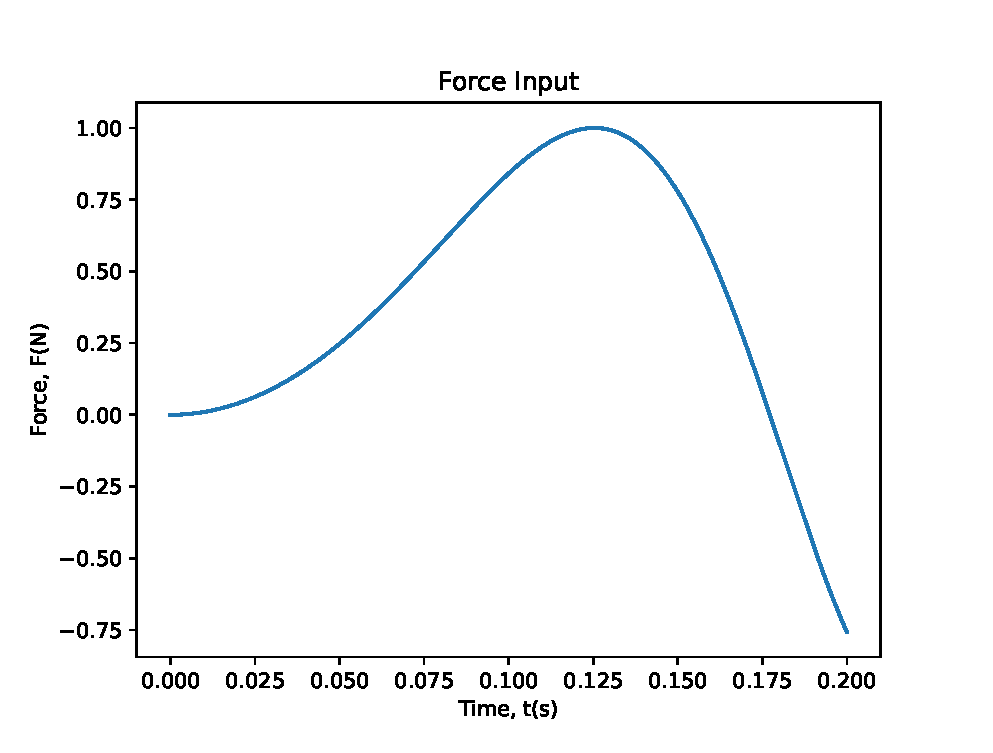
\includegraphics[width=11cm, height=8.25cm]{Force_Input.eps}
\caption
{This graph shows the Force applied to the system over 0.2s.}
\end{figure}

\begin{figure}[H]
\centering
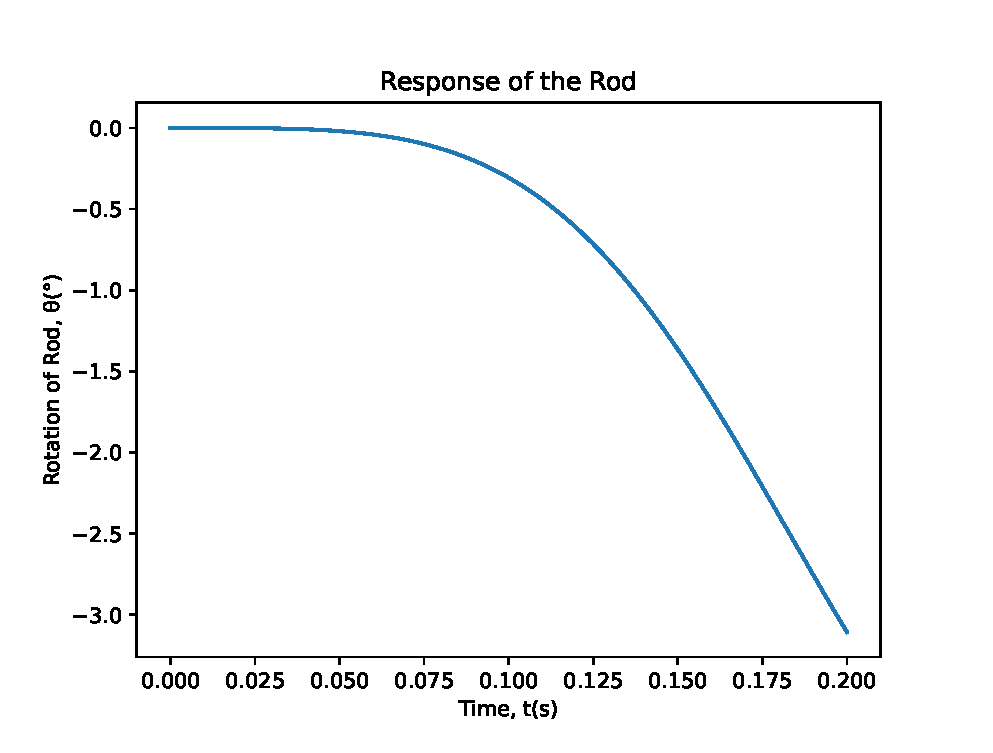
\includegraphics[width=11cm, height=8.25cm]{Response_Rod.eps}
\caption
{This graph shows how the rod rotates, when the force is applied. The rod rotates in an anti-clockwise direction. This is to be expected, as the rotation of the rod was initially at 0\degree, and when the force  is applied, it would expected be to fall in the opposite direction to the force.}
\end{figure}

\begin{figure}[H]
\centering
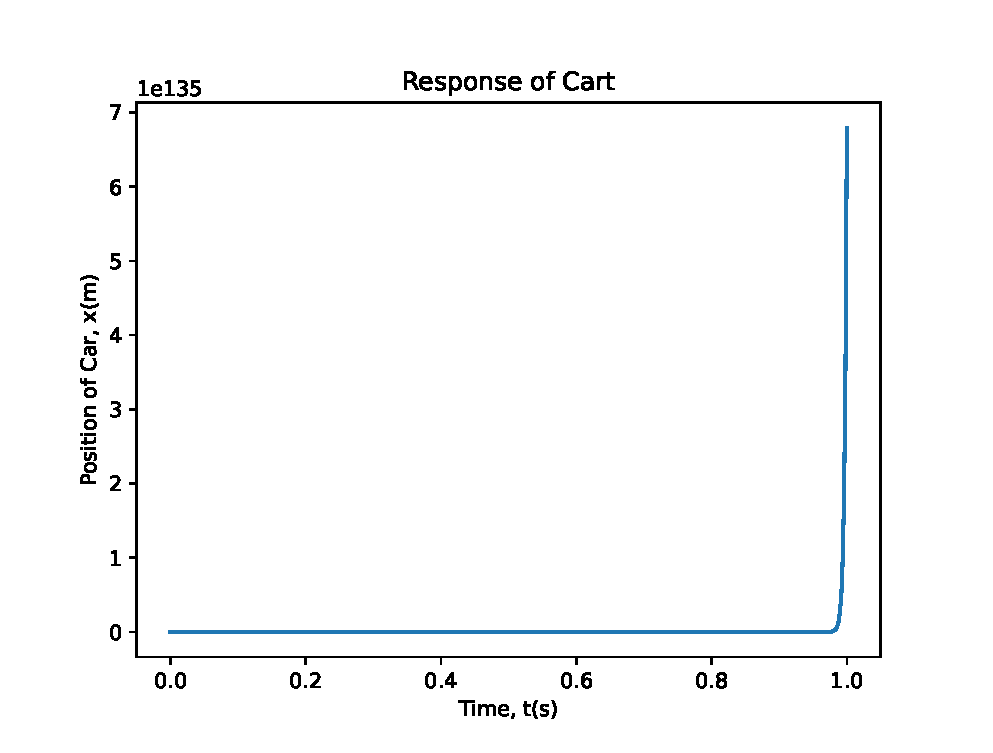
\includegraphics[width=11cm, height=8.25cm]{Response_Cart.eps}
\caption
{The graphs show how the car moves in the x-axis, when the force is applied. It can be seen that it is accelerating away from 0m. This is to be expected, as force is directly proportional to acceleration.}
\end{figure}


\newpage
\section{Question 5}
The following code was created, to make the Rod return as close as possible to the equilibrium position, in the shortest amount of time. PID controls were implemented. These were then used as a feedback control to the system.
\begin{lstlisting}[language=Python]
# Creating a Control PID Controller
def pid(kp, kd, ki, ts):
    return ctrl.TransferFunction([kd / ts, kp, ki * ts], [1, 0])

# Finds the element number which first passes split_var
def elementAt(arr, split_val):
    for x in range(len(arr)):
        if (arr[x] >= split_val):
            return x


t_final = 1  # Simulate for 1s
num_points = 501
time_span = np.linspace(0, t_final, num_points)
cutAt = elementAt(time_span, 0.4)
ts = 1.0 / 501.0

plot_number = 0  # Counts the number of graphs plotted
best_range = 100  # Keeps track of current best values
best_solution = [0, 0, 0]  # Values of the current best PID values

# Keeps track of the difference between maximum and minimum 
# deviation from equilibrium position
ranges = []

test_values = [0.1, 1, 10, 100, 10 ** 3]

for kp in test_values:
    for kd in test_values:
        for ki in test_values:
            # -ve for Negative Feedback.
            controller = -pid(kp, kd, ki, ts)  # PID Controller

            # PID Controller Inputting to Rod
            theta_closed = ctrl.feedback(theta_tf, controller)

            # Kick the system
            t_imp, theta_imp = ctrl.impulse_response(theta_closed,
            							 T=time_span)

            theta_imp = np.rad2deg(theta_imp)  # Convert degrees to radians

            # Filtering

            # Valid Solution must only have peaks at -0.5 and 0.5
            if (not (max(theta_imp) > 5 or min(theta_imp) < -5)):
                theta2_imp = theta_imp[cutAt:]

                # After t=0.4, Valid Solution must only have peaks 
                # at 0 and 0.1
                if (not (max(theta2_imp) > 0.1 or min(theta2_imp) < 0)):
                    range = max(theta_imp) - min(theta_imp)

                    # Plot the graph only if it has better characteristics
                    if (range < best_range):
                        best_range = range
                        plt.plot(t_imp, theta_imp,
                        		label=f"[{kp}, {kd}, {ki}]")
                        # plt.title(f"[{kp} {kd} {ki}] : {range}")
                        # plt.show()
                        plot_number += 1
                        print(f"{plot_number} : [{kp}, {kd}, {ki}] : {range}")
                        best_solution = [kp, kd, ki]
                        ranges.append(range)
                        
print(best_solution)
\end{lstlisting}

\begin{figure}[H]
\centering
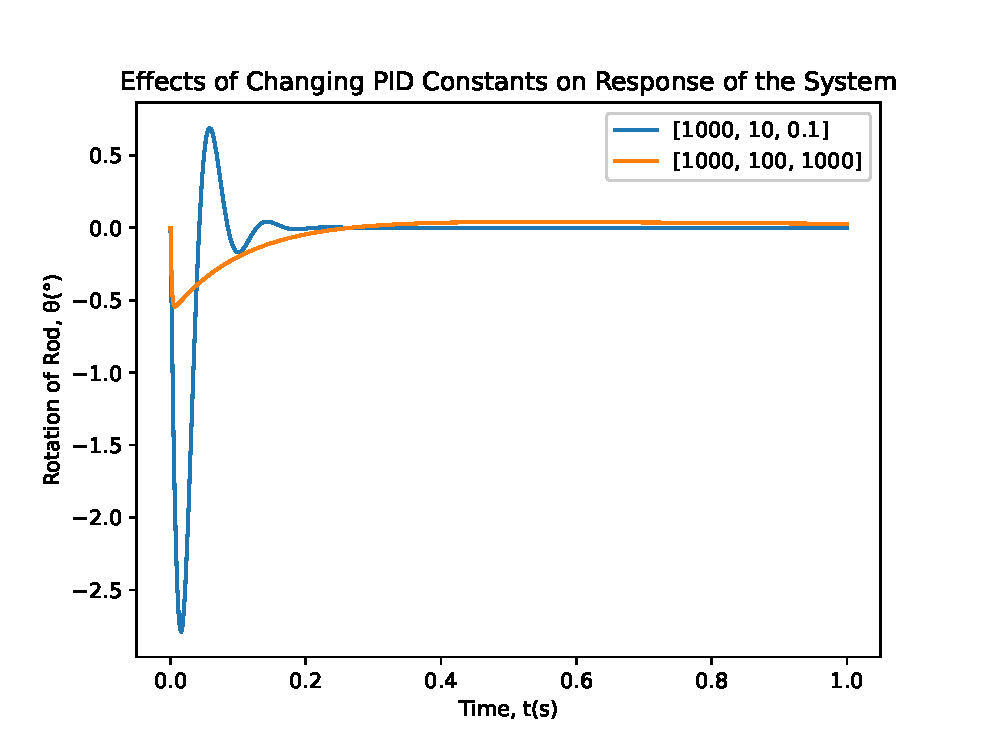
\includegraphics[width=11cm, height=8.25cm]{Changing_PID_Constants.eps}
\caption
{The graphs show how different values of kp, kd, ki, generate different results. The PID values were chosen by the program. Each set of values is better than it's predecessor. As can be seen the the graph, the range of values spanned by each result is subsequently less.}
\end{figure}

\begin{figure}[H]
\centering
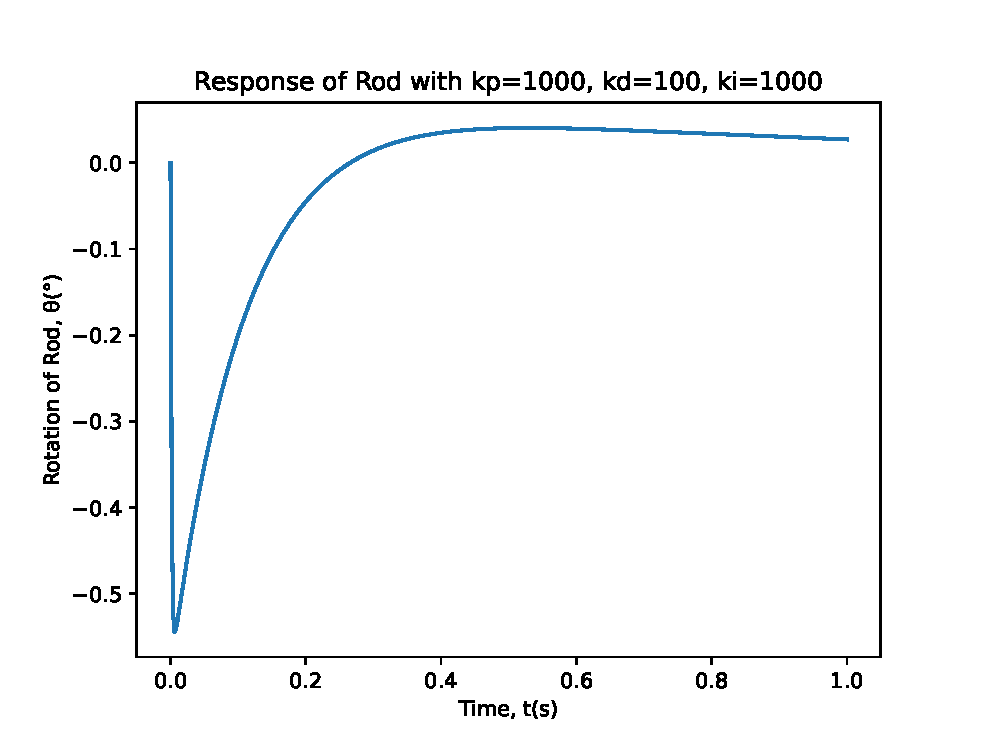
\includegraphics[width=11cm, height=8.25cm]{Best_Solution.eps}
\caption
{This graph shows the result produced by the best PID values. As can be seen from the graph, it is very quick. The range of values it spans is 0.6\degree. This is well within the parameters set, of [-5\degree, 5\degree]. After 0.4s, it is well below 0.1\degree. }
\end{figure}

\newpage
\section{Question 6}
\subsection{Part 1}
The code in Question 5 was modified, so that the PID controls were controlling the cart instead of the rod.
\begin{figure}[H]
\centering
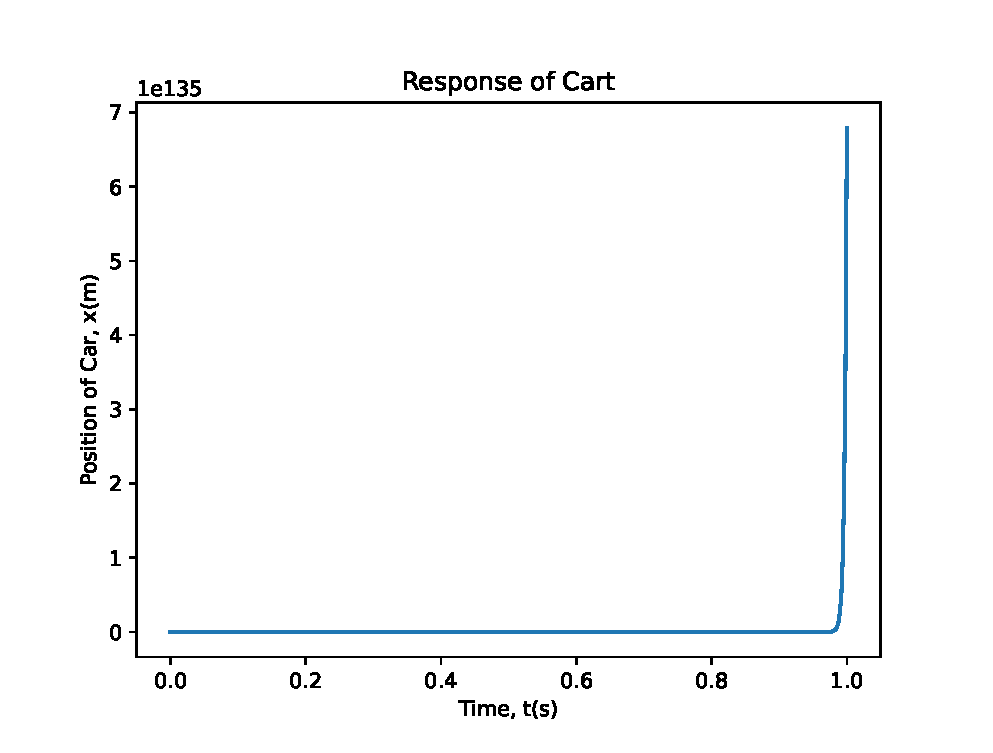
\includegraphics[width=11cm, height=8.25cm]{Response_Cart.eps}
\caption
{This graph shows the result produced by the system. As can be seen from the graph, the car acclereates rapidly towards, $1 \times 10^{135}$m.}
\end{figure}

\noindent
The quirky behavoiur on the graph can be explained by looking at the Transfer Function of the combined PID Controller and $G_x$. \\

\noindent
System Transfer Function $ = \frac{2060 s^5 - 4.33e+04 s^3}{669.4 s^7 - 2.06e+05 s^6 - 2.077e+06 s^5 + 2.27e+06 s^4 + 4.33e+07 s^3 + 4.33e+07 s^2}$\\

\noindent
When the poles of the Transfer Function is determined, it can be seen that it has positive real poles. This means the overall system is unstable. Thsi explains why the cart accelerates towards $1 \times 10^{135}$m.\\
This system could be made stable, by somehow getting all the pole from the positive real side, and shiting them left, so that they are all on the negative real side.

\newpage
\subsection{Part 2}
The code from the Lane Keeping Lab was modified, to produce the following graph. It is very diffficult to work strictly in the time domain.
\begin{figure}[H]
\centering
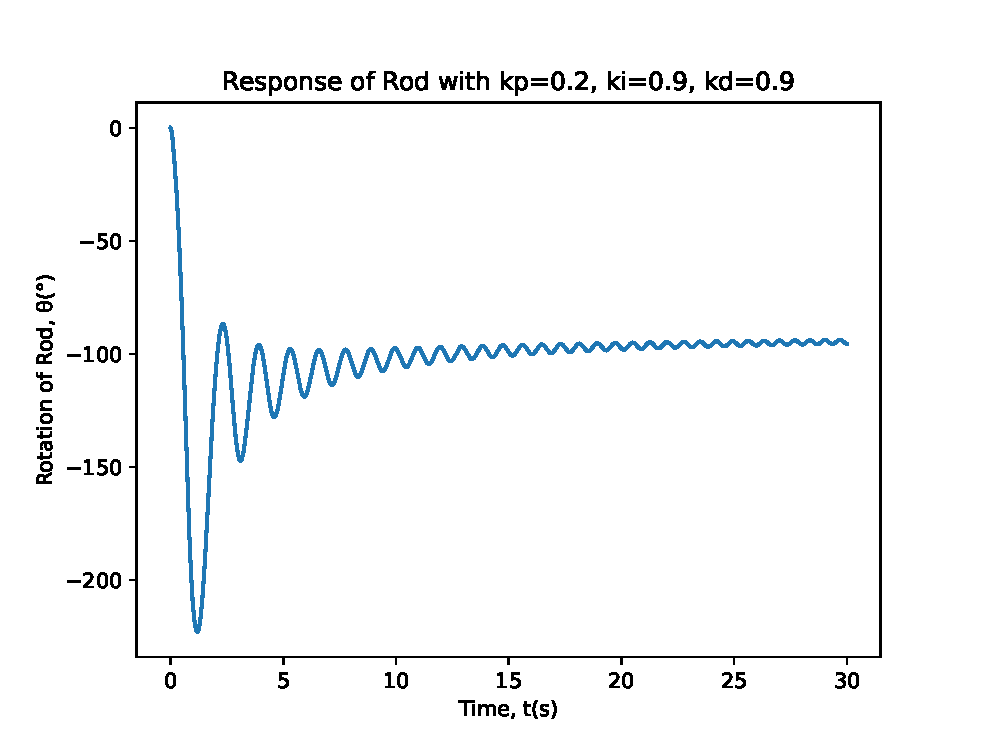
\includegraphics[width=11cm, height=8.25cm]{Response_Rod_t.eps}
\caption
{This graph shows the result produced by PID controller controlling the rod. The graph was obtained, by simulating the non-linear system, where as in Question 5, the linear system, and it's Transfer Function was used.}
\end{figure}

\noindent
No matter what PID values I choose, the rotation of the rod always converged at a value of $k \times 360\degree + 100\degree$, where k is any whole number. For this reason, I could not get it to meet the requirements set out in Question 5.\\

\begin{figure}[H]
\centering
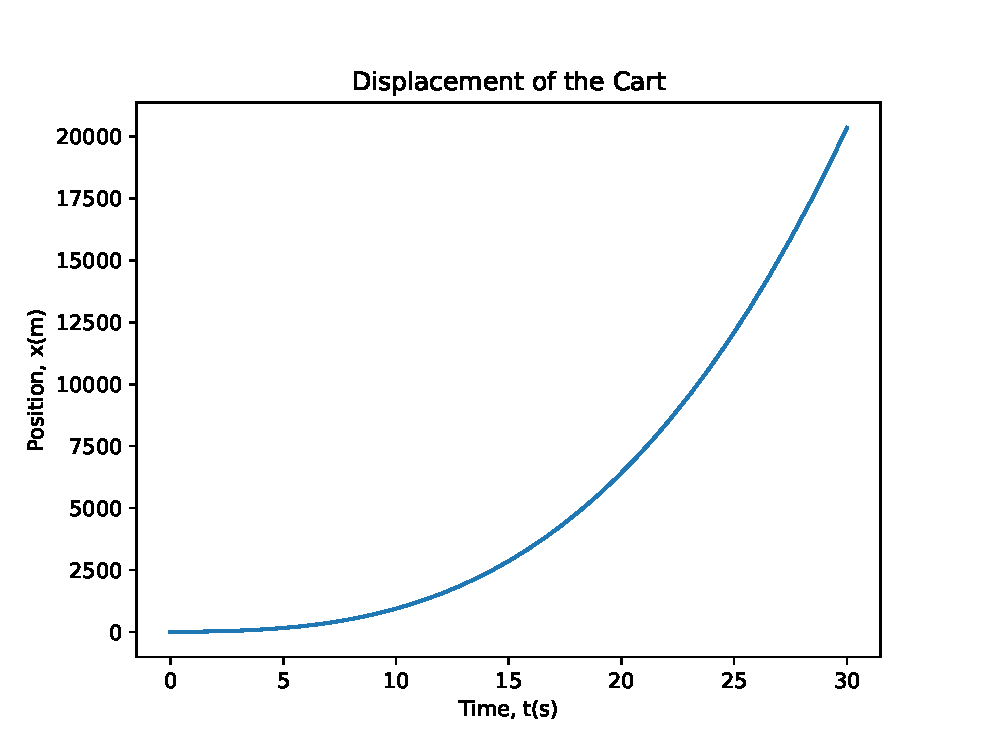
\includegraphics[width=11cm, height=8.25cm]{Q6_pos.eps}
\caption
{This graph shows how the displacement of the cart varies with time. As can be seen from the graph, the cart does 20km in 30s. And it doesn't seem to be slowing down.}
\end{figure}

\begin{figure}[H]
\centering
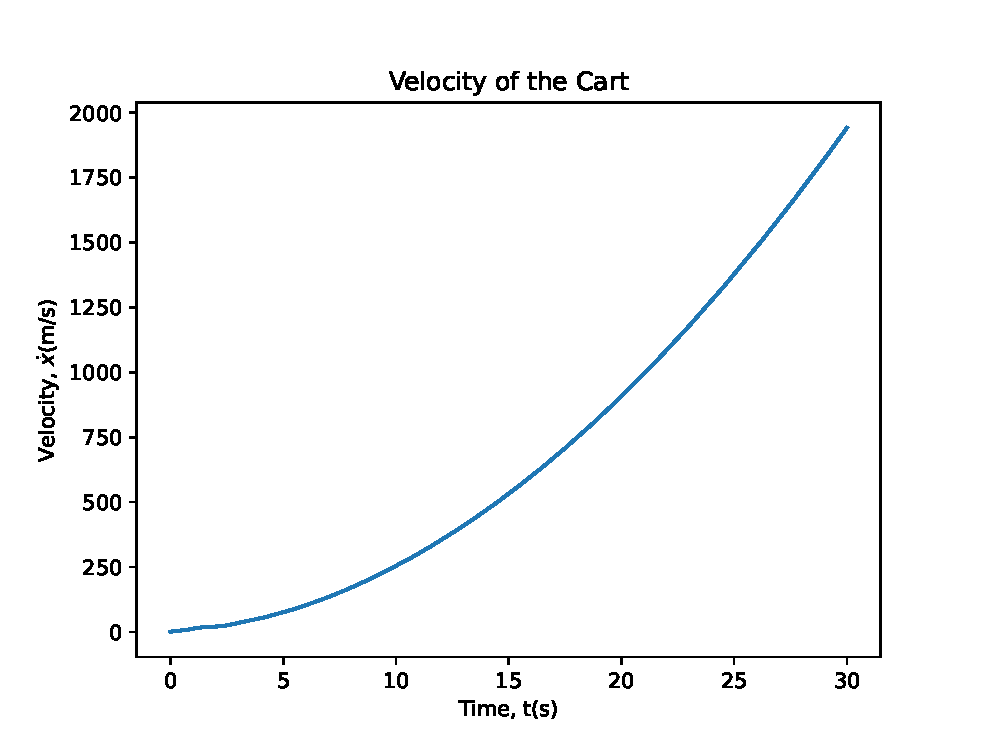
\includegraphics[width=11cm, height=8.25cm]{Q6_vel.eps}
\caption
{This graph shows how the velocity of the cart varies with time. As can be seen from the graph, at the end of 30s, the cart is at a speed of 2km/s. The average acceleation during this time can be approximated to 66.6km/$s^2$}
\end{figure}

\noindent
Taking a value of acceleration at 66.6km/$s^2$, and mass of the system as 0.4kg. The force exerted on the system, can be seen to be 26.7kN.\\

\noindent
The convergence to a $k \times 360\degree + 100\degree$ is very peculiar. But it seems to indicate, that the car is moving too fast, and that the force caused by the acceleration prevents it from propping up the rod any further.\\

\noindent
It therefore seems, that to make the rod converge to a rotation 0\degree, the position of the cart needs to be restricted to a closed space, and the velocity of the cart should be limited to a maximum value.


\end{document}



















